\documentclass[10pt,a4paper]{article}
\usepackage[utf8]{inputenc}
\usepackage{amsmath}
\usepackage{gensymb}
\usepackage{amsfonts}
\usepackage{siunitx}
\usepackage[european]{circuitikz}
\usepackage{geometry}
\newgeometry{tmargin=2cm, bmargin=2cm, lmargin=2cm, rmargin=2cm}
\usepackage{amssymb}
\usepackage{polski}
\usepackage{graphicx}
\author{\textbf{T. Fąs}}
\title{\textbf{WSPÓŁCZYNNIKI ZAŁAMANIA W RUTYLU}}
\begin{document}
\maketitle

\begin{center}
\textbf{\subsection*{STRESZCZENIE}}
\end{center}
W doświadczeniu wyznaczono zależność współczynników załamania światła od długości fali dla promienia zwyczajnego i nadzwyczajnego w uproszczonym modelu Sellmeiera postaci $n^2-1=B_{i}\lambda^2/(\lambda^2-C_{i})$. Otrzymano wartości: dla promienia zwyczajnego $B_{z}=5,0929\pm0,0083$ 1/nm$^2$, $C_{z}=46524\pm432$ nm$^2$, dla promienia nadzwyczajnego: $B_{n}=6,309\pm0,038$ 1/nm$^2$, $C_{n}=51692\pm1564$ nm$^2$.


\begin{center}
\textbf{\subsection*{WSTĘP}}
\end{center}
Kryształ rutylu $-$ TiO$_{2}$ $-$ jest kryształem wykazującym dwójłomność. W związku z tym promień padający na taki kryształ ulega rozdzieleniu na promień zwyczajny i nadzwyczajny, o różnych właściwościach. Zależność współczynnika załamania dla kryształu rutylu jest inna dla promienia zwyczajnego i nadzwyczajnego. Celem doświadczenia było znalezienie tej zależności dla obu promieni. 


\begin{figure}[h!]
\centering
\begin{minipage}{0.5\textwidth}
  \centering
  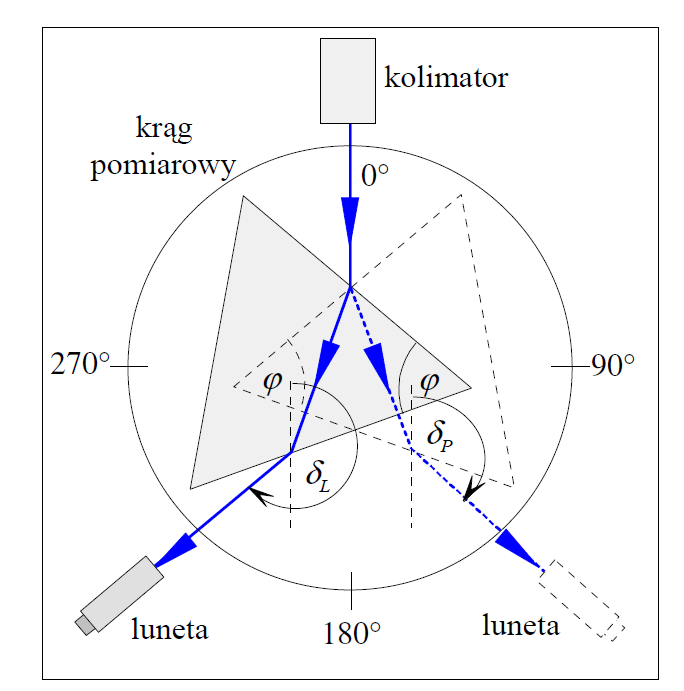
\includegraphics[width=6cm, height=5cm ]{rap13ukl1} 
\caption{Wyznaczanie kąta najmniejszego odbicia.}
\end{minipage}%
\begin{minipage}{0.5\textwidth}
  \centering
  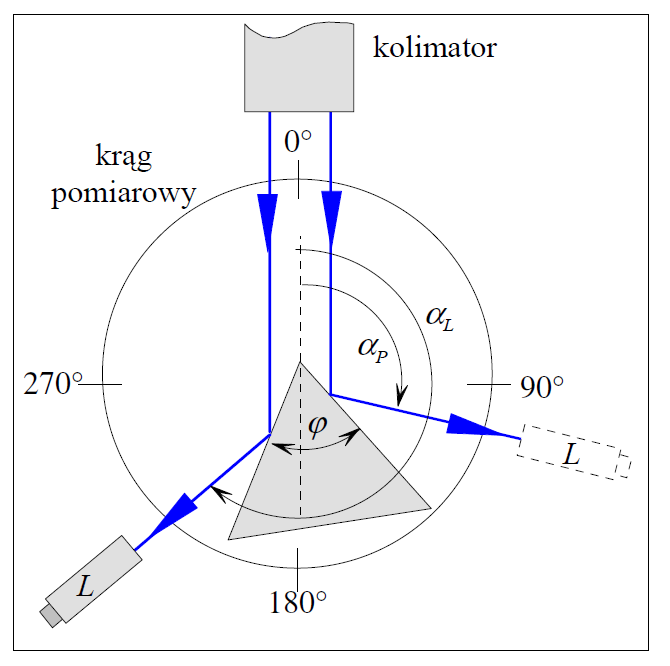
\includegraphics[width=6cm, height=5cm ]{rap13ukl2} 
\caption{Wyznaczanie kąta łamiącego.}
\end{minipage}
\end{figure}



Jeżeli promień pada na kryształ tak, jak na Rysunku 1, to współczynnik załamania $n$ można wyznaczyć, korzystając z prawa Snella. Jeżeli znamy kąt najmniejszego odbicia $\delta$ oraz kąt łamiący pryzmatu $\varphi$, to $n$ wyrażone jest wzorem:
\begin{equation}
n=\dfrac{\sin\left(\dfrac{1}{2}\left(\delta+\varphi\right)\right)}{\sin\left(\dfrac{1}{2}\varphi\right)},
\end{equation}
przy czym zachodzi równość:
\begin{equation}
\delta=\dfrac{1}{2}\left(\delta_{l}-\delta_{p}\right).
\end{equation}
Z kolei z Rysunku 2 wynika, iż kąt łamiący pryzmatu można wyznaczyć ze związku 
\begin{equation}
\varphi=\dfrac{1}{2}\left(\alpha_{l}-\alpha_{p}\right).
\end{equation}

 Jeżeli znane są rożne wartości współczynników $n$ dla rożnych długości fali $\lambda$, to można do tych danych dopasować zależność:
\begin{equation}
n=A_{0}+\dfrac{A_{1}}{\lambda^2},
\end{equation}
lub
\begin{equation}
n^2-1=\dfrac{B_{1}\lambda^2}{\lambda^2-C_{1}},
\end{equation}
przy czym $A$, $B$, $C$ to współczynniki dopasowania.

\begin{center}
\textbf{\subsection*{UKŁAD DOŚWIADCZALNY}}
\end{center}

Do pomiarów kątów skorzystano z goniometru, a źródłem światła była lampa sodowa i rtęciowa. Goniometr w trakcie pomiarów był ustawiany zgodnie z Rysunkiem 1 i Rysunkiem 2. 
Do rozróżnienia promienia zwyczajnego od nadzwyczajnego wykorzystano polaryzator.

\begin{center}
\textbf{\subsection*{WYNIKI POMIARÓW}}
\end{center}
Zmierzono: $\alpha_{p}=140^{\circ}01'$, $\alpha_{l}=200^{\circ}20'$. Tabela 1 przedstawia pomiary kątów $\delta_{l}$ i $\delta_{p}$ wraz z powiązanymi z nimi długościami fali. 

\begin{table}[h!]
\centering
\caption{Kąty załamania.}
\begin{tabular}{|c|c|c|c|c|}
\hline
Długość fali $\lambda$ [nm] & 589,3          & 650,0          & 546,1          & 404,1          \\ \hline
$\delta_{p}$ (zwyczajny)    & 123$^\circ$33' & 125$^\circ$10' & 122$^\circ$59' & 114$^\circ$29' \\ \hline
$\delta_{l}$                & 247$^\circ$46' & 234$^\circ$20' & 236$^\circ$56' & 245$^\circ$27' \\ \hline
$\delta_{p}$ (nadzwyczajny) & 112$^\circ$14' & 113$^\circ$03' & 109$^\circ$55' & 97$^\circ$33'  \\ \hline
$\delta_{l}$                & 235$^\circ$23' & 246$^\circ$55' & 249$^\circ$54' & 262$^\circ$20' \\ \hline
\end{tabular}
\end{table}

\begin{center}
\textbf{\subsection*{ANALIZA DANYCH}}
\end{center}
Niepewność pomiarów kątów $\alpha_{l}$ i $\alpha_{p}$ oszacowano na $\Delta_{\alpha}=1'$. Z kolei niepewności kątów $\delta_{i}$ przyjęto jako równe $\Delta_{\delta}=5'$, ponieważ uchwycenie momentu, w którym dochodzi do cofania się obrazu kolimatora jest trudne. Również goniometr nie był idealnie wypoziomowany, co mogło zaburzyć niektóre pomiary.

Aby przenieść te niepewności na niepewności kąta łamiącego i kąta najmniejszego odchylenia, skorzystano z metody propagacji małych błędów. Ogólny wzór przenoszenia niepewności w tej metodzie jest następujący:

 \begin{equation}
 u_{f}^2=\sum_{i=1}^n \left( \dfrac{\partial f}{\partial x_{i}}u_{i}\right)^2+\sum_{i=1, i\neq j}^n \left( \dfrac{\partial f}{\partial x_{i}}\dfrac{\partial f}{\partial x_{j}}c_{ij}\right),
 \end{equation}
 gdzie wielkość $f$ zależy od wielkości $x_{i}$ o niepewnościach $u_{i}$ i o ocenach kowariancji $c_{ij}$ \cite{tay1}. W przypadku mierzonych kątów, kowariancja między nimi wynosi 0.

Stosując dane z Tabeli 1 oraz Równanie (6) wyznaczono kąt łamiący pryzmatu $\varphi=(30,158\pm0,012)^\circ$ oraz współczynniki załamania $n_{z}$ i $n_{n}$ dla kolejno promienia zwyczajnego i nadzwyczajnego wraz z ich niepewnościami $u_{i}$. Wyniki umieszczono w Tabeli 2.
\begin{table}[h!]
\centering
\caption{Współczynniki załamania i ich niepewności.}

\begin{tabular}{|c|c|c|c|c|}
\hline
Długość fali $\lambda$ [nm] & 589,3 & 650,0 & 546,1 & 404,7 \\ \hline
$n_{z}$                       & 2,623 & 2,590 & 2,649 & 2,849 \\ \hline
$u_{nz} $                     & 0,099 & 0,102 & 0,102 & 0,099 \\ \hline
$n_{n}   $                    & 2,899 & 2,881 & 2,948 & 3,197 \\ \hline
$u_{nn}   $                   & 0,102 & 0,099 & 0,098 & 0,095 \\ \hline
\end{tabular}
\end{table}

Otrzymane współczynniki dla linii widmowej sodu $\lambda=589,3$ nm są zgodne ze współczynnikami wzorcowymi, które wynoszą odpowiednio $n_{z}=2,61$, $n_{n}=2,910$ \cite{wd}. Zgodność zbadano za pomocą testu $3\sigma$, czyli sprawdzono, czy różnica wyników jest mniejsza od trzykrotnej niepewności tej różnicy.


W następnym kroku, korzystając z programu \textit{gnuplot} wykonano dopasowanie danych z Tabeli 2 zgodnie z Równaniem (4). Krzywe najlepszego dopasowania są przedstawione na Rysunku 3 i Rysunku 4, a parametry dopasowania wraz z ich niepewnościami $u_{i}$ przedstawione są w Tabeli 3.


\begin{figure}[h!]
\centering
\begin{minipage}{0.5\textwidth}
  \centering
  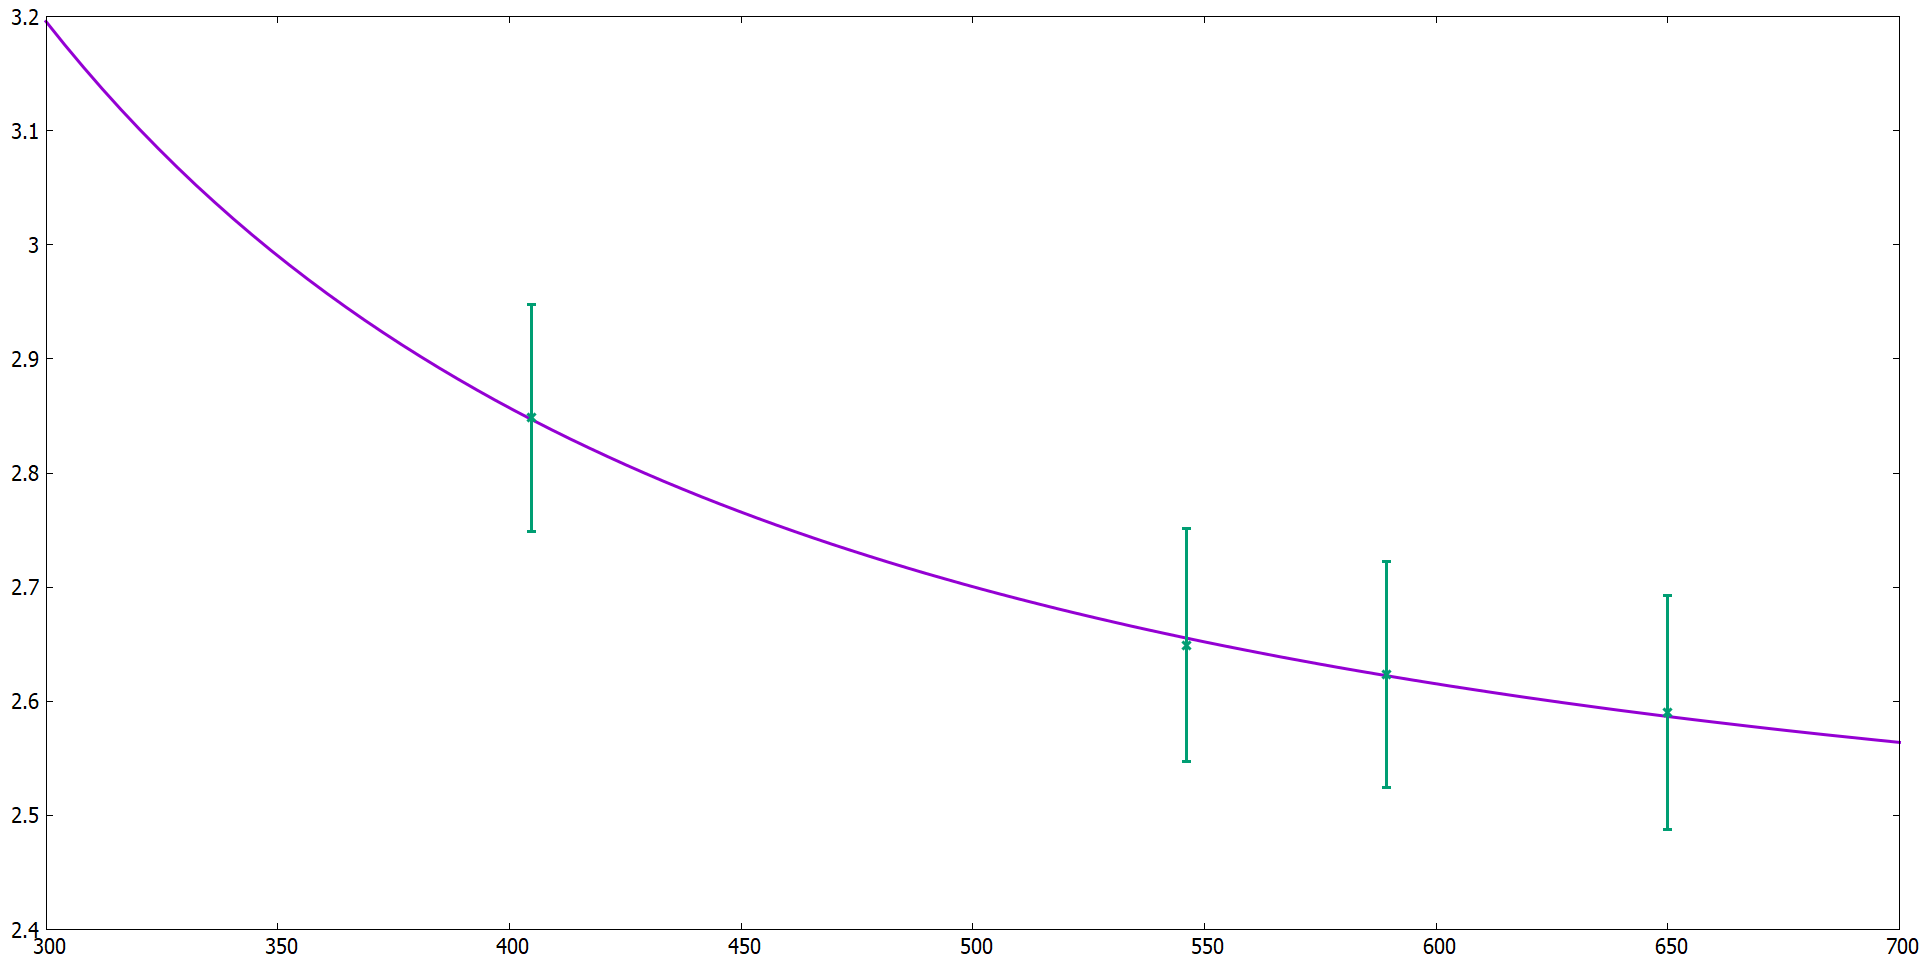
\includegraphics[width=8cm, height=5cm ]{rap13rys1} 
\caption{Dopasowanie danych: promień zwyczajny.}
\end{minipage}%
\begin{minipage}{0.5\textwidth}
  \centering
  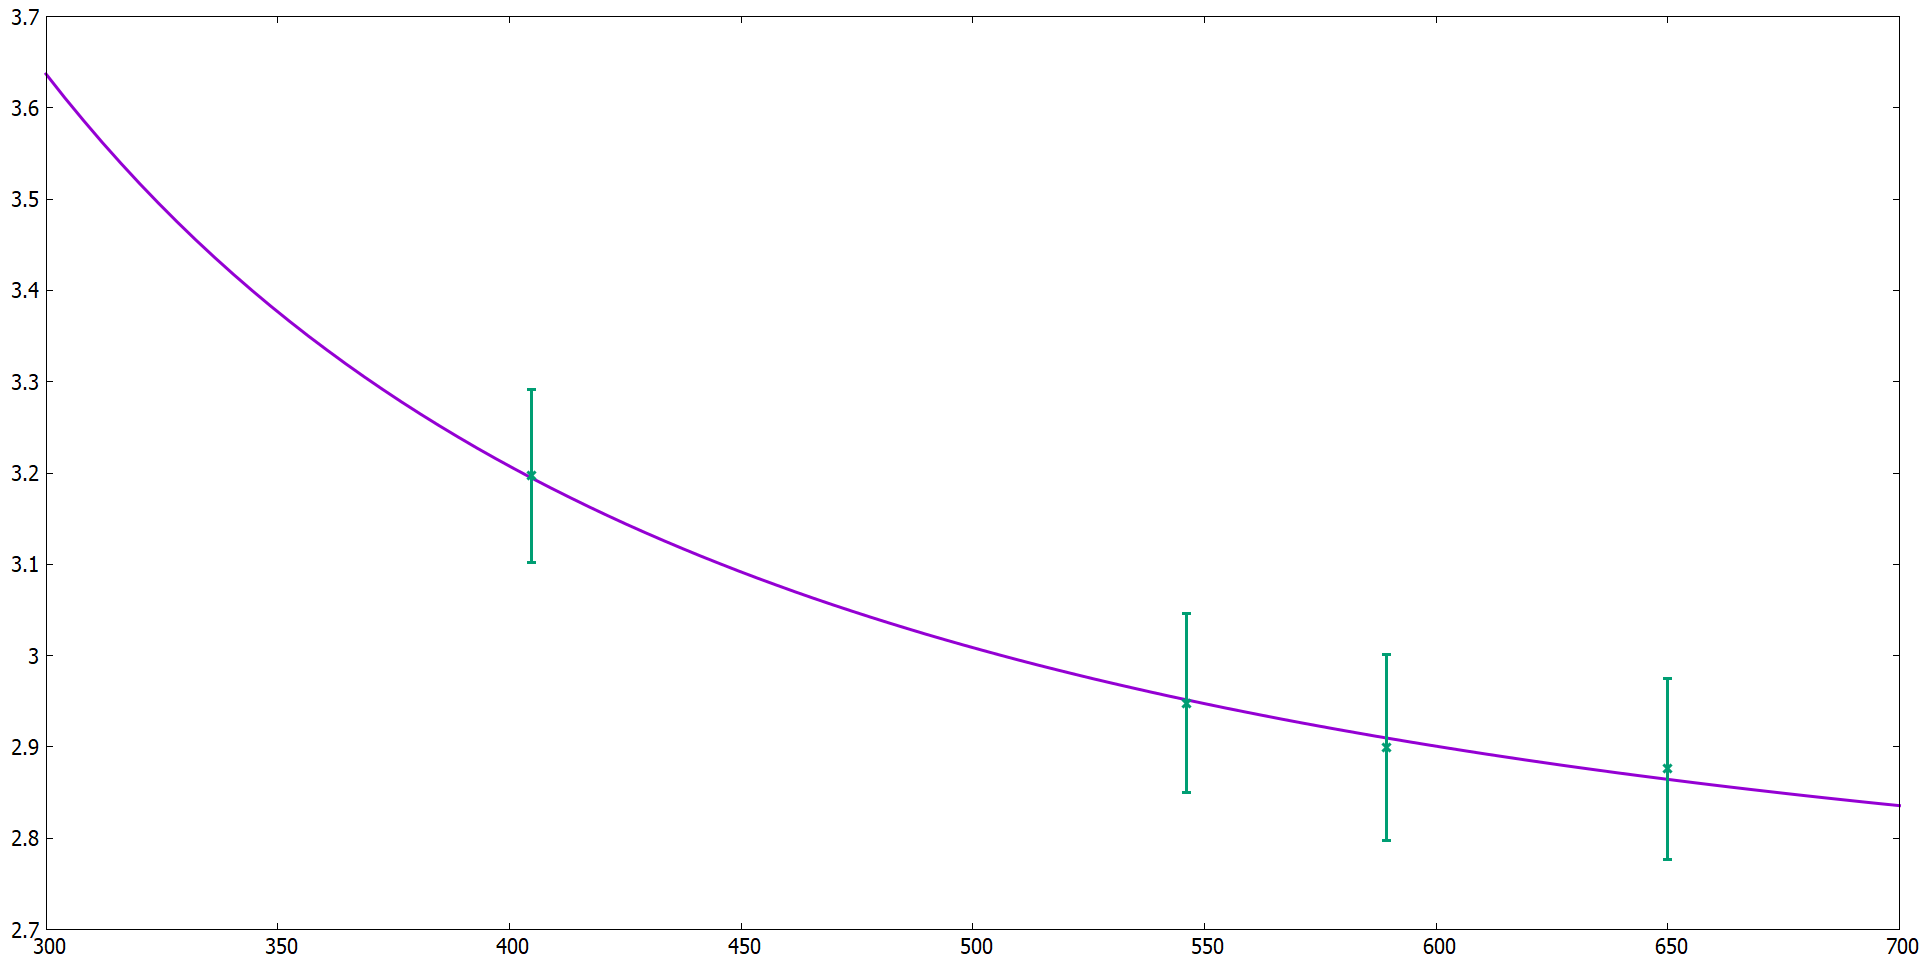
\includegraphics[width=8cm, height=5cm ]{rap13rys2} 
\caption{Dopasowanie danych: promień nadzwyczajny.}
\end{minipage}
\end{figure}


\begin{table}[h!]
\centering
\caption{Parametry dopasowania.}
\begin{tabular}{|c|c|c|c|c|c|}
\hline
Promień      & $A_{0}$ & $A_{1}$ [nm$^2$] & $u_{A0}$ & $u_{A1}$ [nm$^2$] & $\chi^2$ \\ \hline
Zwyczajny    & 2,4234  & 69696          & 0,0050   & 1629              & 0,0028   \\ \hline
Nadzwyczajny & 2,638   & 91080          & 0,015    & 4894              & 0,028   \\ \hline
\end{tabular}
\end{table}


Analogiczną procedurę zastosowano w przypadku dopasowywania danych do Równania (5). Krzywe wynikłe z tego dopasowania przedstawiono na Rysunku (5) i Rysunku (6), a parametry dopasowania są przedstawione w Tabeli 4.

\begin{figure}[h!]
\centering
\begin{minipage}{0.5\textwidth}
  \centering
  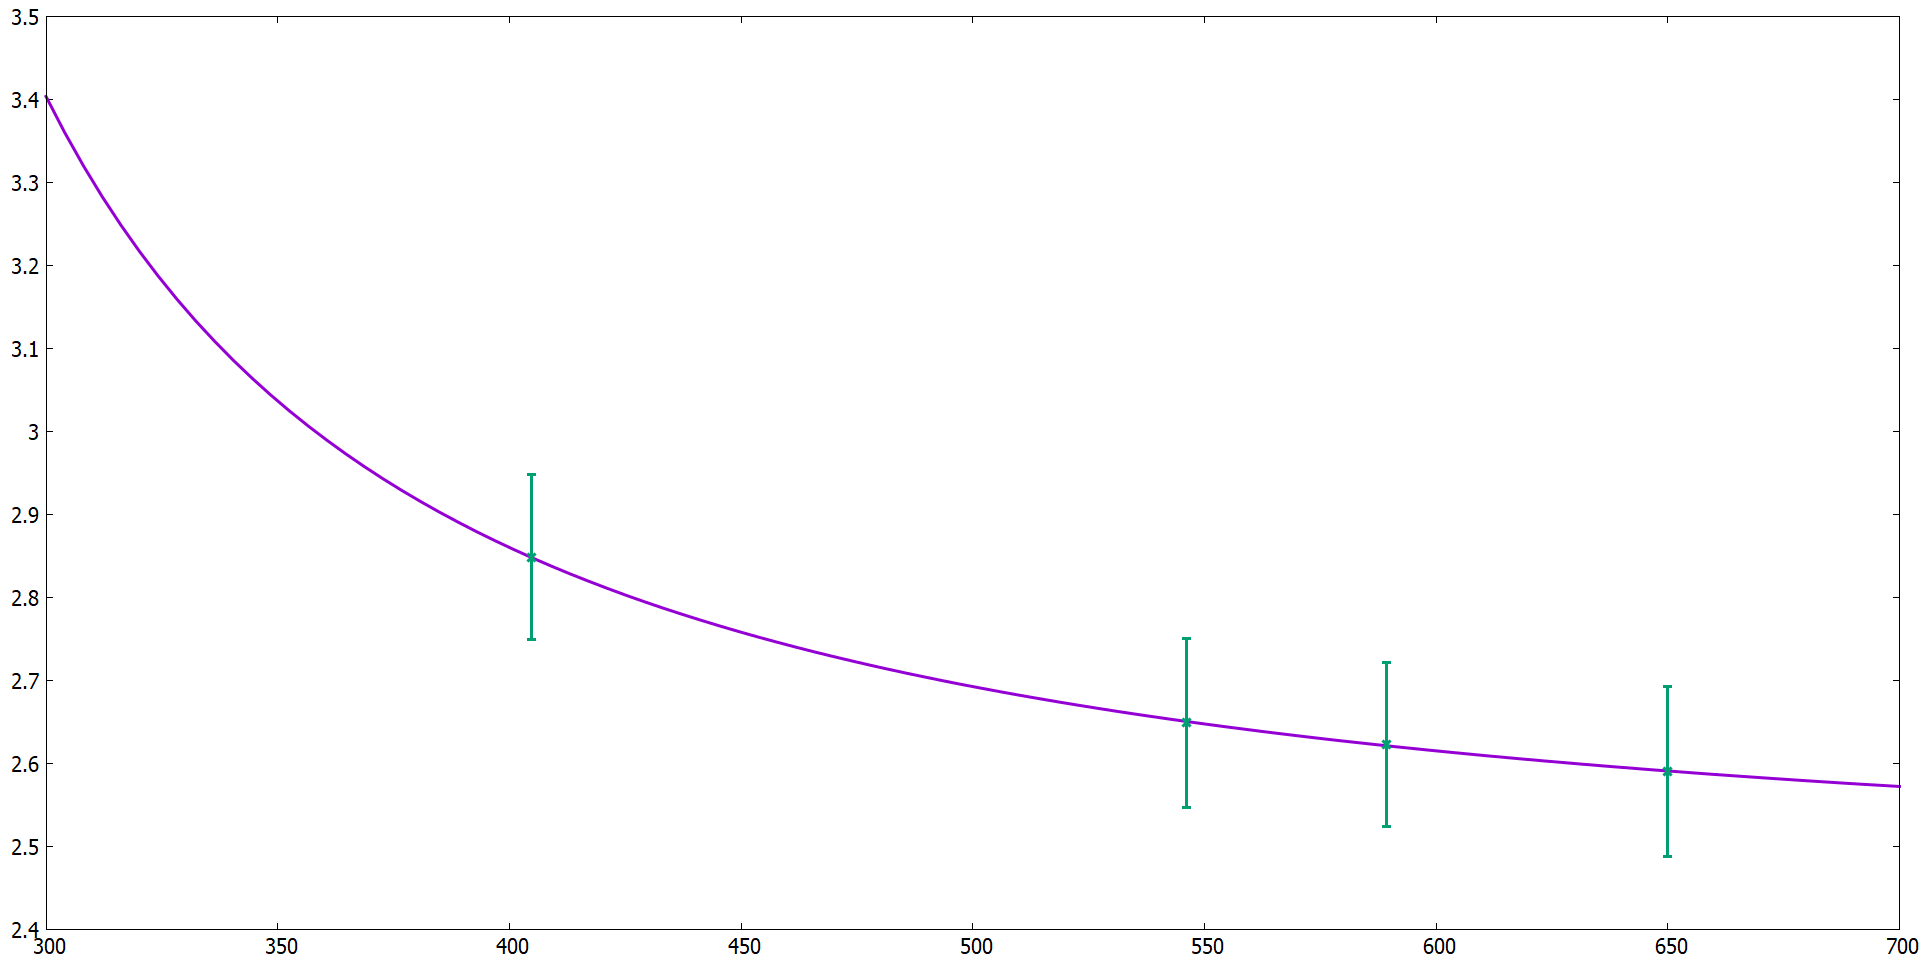
\includegraphics[width=8cm, height=5cm ]{rap13rys3} 
\caption{Dopasowanie danych: promień zwyczajny.}
\end{minipage}%
\begin{minipage}{0.5\textwidth}
  \centering
  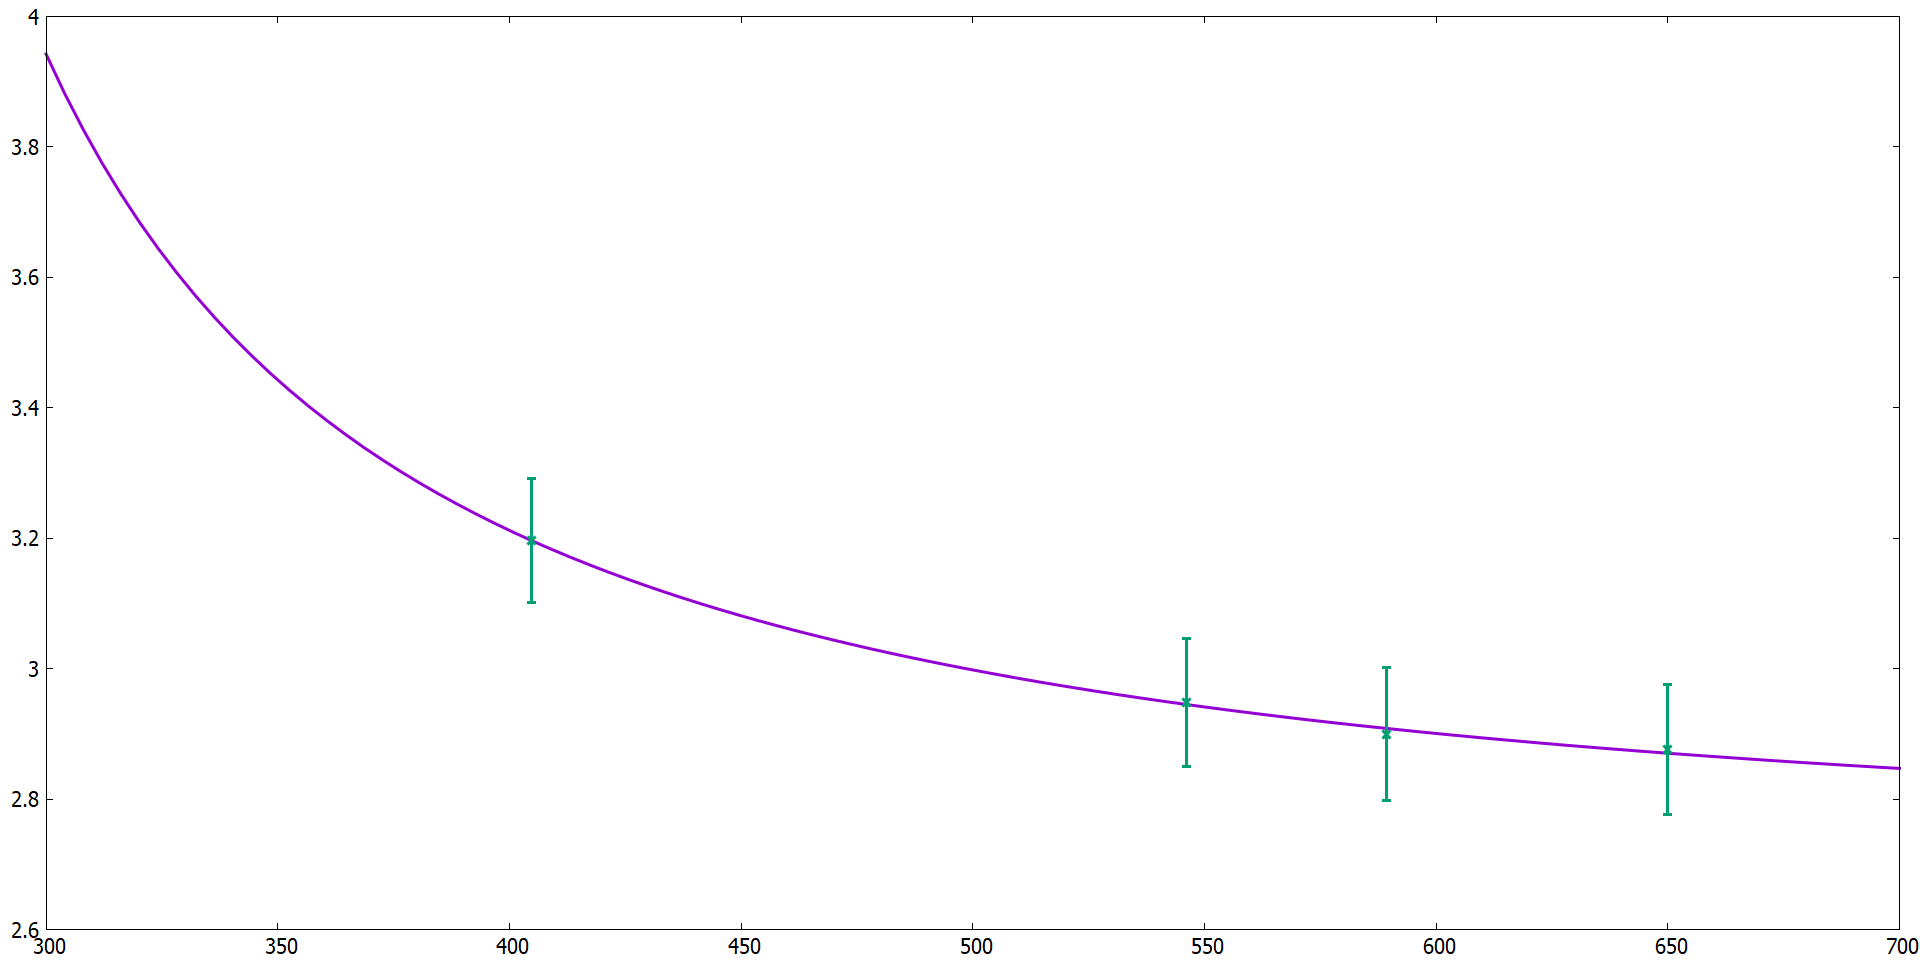
\includegraphics[width=8cm, height=5cm ]{rap13rys4} 
\caption{Dopasowanie danych: promień nadzwyczajny.}
\end{minipage}
\end{figure}


\begin{table}[h!]
\centering
\caption{Parametry dopasowania.}
\begin{tabular}{|c|c|c|c|c|c|}
\hline
Promień      & $B_{1}$ [1/nm$^2$] & $C_{1}$ [nm$^2$] & $u_{B1}$ [1/nm$^2$] & $u_{C1}$ [nm$^2$] & $\chi^2$ \\ \hline
Zwyczajny    & 5,0929  & 46525            & 0,0084   & 432               & 0,00077  \\ \hline
Nadzwyczajny & 6,308   & 51693            & 0,038    & 1564              & 0,017    \\ \hline
\end{tabular}
\end{table}

Otrzymane wartości $\chi^2$ sugerują, iż zależność wyrażona Równaniem (5), czyli model Sellmeiera, jest lepszym odwzorowaniem faktycznie uzyskiwanych wyników.



\begin{center}
\textbf{\subsection*{DYSKUSJA WYNIKÓW I WNIOSKI}}
\end{center} 
Dysponując gotową krzywą kalibracyjna, można odwrócić zależność wyrażoną przez Równanie (5) by uzyskać zależność pozwalającą na wyznaczanie długości fali przy znajomości współczynnika załamania. W ten sposób otrzymano spektroskop. Jednak nie przeprowadzono tej procedury w analizie danych, gdyż ze względu na małą liczbę punktów zdecydowano się włączyć współczynniki załamania sodu do analizy kalibracyjnej. Jednak niezwykle niskie wartości $\chi^2$ jak i niskie wartości niepewności współczynników pozwalają sądzić, iż otrzymane długości fali byłyby zgodne z wartościami rzeczywistymi jak i byłyby obarczona małymi niepewnościami.

\begin{center}
\begin{thebibliography}{9}

 
\bibitem{tay1}
 J. R. Taylor,
 \emph{Wstęp do analizy błędu pomiarowego},
 PWN, Warszawa, 1995, s. 175.
 
  \bibitem{wd}
 J. R. DeVore,
 \emph{Refractive Indices of Rutile and Sphalerite},
OSA, 06.1951, t. 41 s. 416--419. 


 \end{thebibliography}

\end{center}


\end{document}